\documentclass{article} 

%----------PACKAGES----------   
    \usepackage[utf8]{inputenc} %just do it
    \usepackage[english]{babel}
    \usepackage{graphicx} %allows images
        \graphicspath{documents/}
    \usepackage{amsmath} %allows maths equations
    \usepackage{geometry} %allows editing of page geometry (https://www.overleaf.com/learn/latex/Page_size_and_margins)
        \geometry{
            a4paper,
            top=0.7in,
            bottom=1in,
            textwidth=7in
            }
    \usepackage{sectsty} %alter section title formatting
        \sectionfont{\fontsize{13}{16}\selectfont}
    \usepackage{tabularx}
    \usepackage[table]{xcolor}
    \usepackage{enumitem}
    \usepackage{color, colortbl}
    \usepackage{tikz}                   
    \usetikzlibrary{shadows}
    \usepackage{transparent}
    \usepackage[framemethod=tikz]{mdframed}
    \usepackage{lipsum}
    \usepackage{tikz,lipsum,lmodern}
    \usepackage[most]{tcolorbox}
    \usepackage{tikz}
    \usepackage{tabularx}
    \usepackage{array}
    \usepackage{bm} 
%----------\PACKAGES----------   

%----------FORMATTING---------- 
    \title{\textbf{WTTS}}
    \author{Rahul Kakaiya}
    \date{}
    
    \newcommand\customfont[1]{\usefont{'playtime.ttf'}}
    
    \renewcommand{\arraystretch}{3}
    
    
    %-----COLOURS-----
    \definecolor{purple}{RGB}{142, 68, 173}
    \definecolor{blue}{RGB}{52, 152, 219}
    \definecolor{orange}{RGB}{243, 156, 18 }
    \definecolor{red}{RGB}{231, 76, 60}
    \definecolor{turquoise}{RGB}{60, 177, 188}
    \definecolor{dblue}{RGB}{31, 97, 141}
    \definecolor{lblue}{RGB}{21, 204, 236}
    \definecolor{dgreen}{RGB}{22, 137, 45}
    %-----\COLOURS-----
    
    
    \newcommand\invisiblesection[1]{
    \refstepcounter{section}
    \addcontentsline{toc}{section}{\protect\numberline{\thesection}#1}
    \sectionmark{#1}}
    
    \newcommand\invisiblesubsection[1]{
    \refstepcounter{subsection}
    \addcontentsline{toc}{subsection}{\protect\numberline{\thesubsection}#1}
    \sectionmark{#1}}
    
    \newenvironment{white}{\color{white}}{\ignorespacesafterend}
    
    \begin{document}
%----------\FORMATTING---------- 
%
%
%
%
%
% MAIN TEXT
%
%
%
%
%
%----------1. STAR CLUSTERS----------
\invisiblesection{1. Astronomy and Star Clusters}
    
    %---title---
    \begin{tcolorbox}[enhanced,colback=red!80!black,colframe=red!80!black,drop fuzzy shadow]
    \begin{center}  
    {\color{white}
        \Huge{\textbf{1. STARS AND STAR CLUSTERS}}
    }
    \end{center}
    \end{tcolorbox}
    %---\title---
    
    
    
    %---intro box---
    \begin{tcolorbox}[enhanced,colback=red!80!white,colframe=red!80!black]
    {\color{white}
        \textbf{After reading this section, you will be able to answer these questions:}
        \begin{itemize}
        \renewcommand\labelitemi{--}
            \item \textbf{What are star clusters? How are star clusters formed?}
            \item \textbf{What are some unique properties of star clusters which make them so interesting to scientists?}
            \item \textbf{What are Cepheid variable stars?} 
        \end{itemize}
    }
    \end{tcolorbox}
    %---\intro box---
    
    
    


    %---enumerate 1,2---
    \begin{enumerate}[label=\color{red}\theenumi]
        \item Sometimes, stars in the Universe are born so close to each other that the force of gravity holds them tightly together. 
        
        \item Groups of stars like these are known as \emph{\textcolor{orange}{star clusters}}. These stars in a particular cluster are \emph{\textcolor{orange}{born out of the same gas cloud}}.
        
        \begin{itemize}[label=\textcolor{red}{\textbullet}]
            \item There are two types of star clusters; \emph{\textcolor{orange}{open star clusters}} and \emph{\textcolor{orange}{globular star clusters}} (\textbf{figure \ref{open-glob}}).
            
            \item \emph{\textcolor{orange}{Open star clusters}} are younger, less dense, and less tightly bound than globular star clusters.
        \end{itemize}
        
    \end{enumerate}
    %---\enumerate---
    
    
    
    %---figure 1---    
    \begin{figure}[h!]
        \begin{center}
        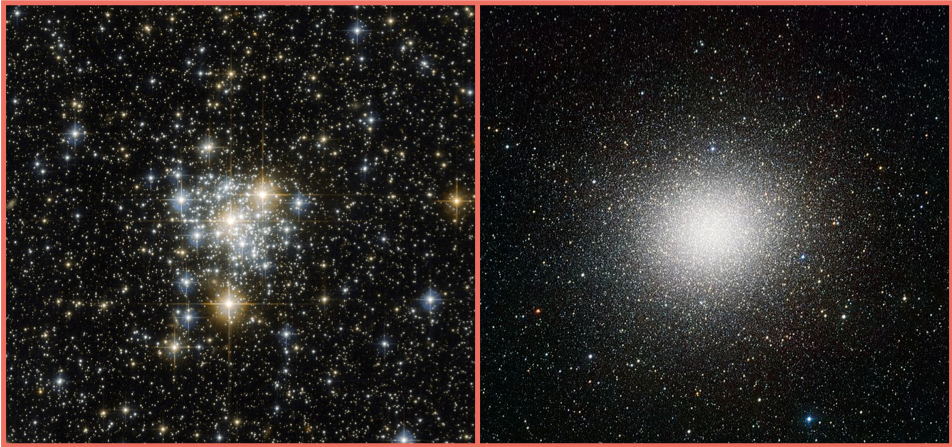
\includegraphics[width=0.7\textwidth]{Images/open-globular.png}
        \textbf{
            \caption{The NGC 299 \emph{\textcolor{orange}{open cluster (left)}}, and the Omega Centauri \emph{\textcolor{orange}{globular cluster (right)}}. Notice how the globular cluster is much denser in stars and more tightly bound than the open cluster.}
        }
        \end{center}
        \label{open-glob}
    \end{figure}
    %---\figure--- 
    
    
    
    %---colourbox 1---
    \begin{tcolorbox}[colback=white,colbacktitle=red!75!white,colframe=red!75!white,title=\textbf{Stars in star clusters are like siblings - they share certain properties...}]
    
        \renewcommand{\theenumi}{\Roman{enumi}}
        \begin{enumerate}
            \item Stars in a star cluster have \emph{\textcolor{orange}{similar chemical compositions}}.
            
            \item Because the stars are so close together, the stars within a given star cluster are all approximately the same distance away from Earth.
            
            \item The main difference between the individual stars in a star cluster is their masses - the \emph{\textcolor{orange}{younger stars are generally smaller and lighter in mass}}, whilst the \emph{\textcolor{orange}{older stars are larger and heavier}}. 
            
            \item Older stars are also generally \emph{\textcolor{orange}{brighter}} than younger stars.
        \end{enumerate}
        
    \end{tcolorbox}
    %---\colourbox---
    
    
    
    %---enumerate 3,4---
    \begin{enumerate}[label=\color{red}\theenumi]
    \setcounter{enumi}{2}
        \item Another type of star in the Universe are \emph{\textcolor{orange}{Cepheid variable stars}}.
        
        \item \emph{\textcolor{orange}{Cepheid variable stars}} are stars which ‘pulsate' with a certain \emph{\textcolor{orange}{period}}, $ \textcolor{red}{\boldsymbol{P}} $. 
        
        
        \begin{itemize}[label=\textcolor{red}{\textbullet}]
            \item In other words, they \emph{\textcolor{orange}{expand and contract with a regular time-period}}, increasing and decreasing in brightness and size (\textbf{figure \ref{cepheid-period}}).
        \end{itemize}
        
        
    \end{enumerate}
    %---\enumerate---
    
    
    
    %---figure 2---    
    \begin{figure}[t!]
        \begin{center}
        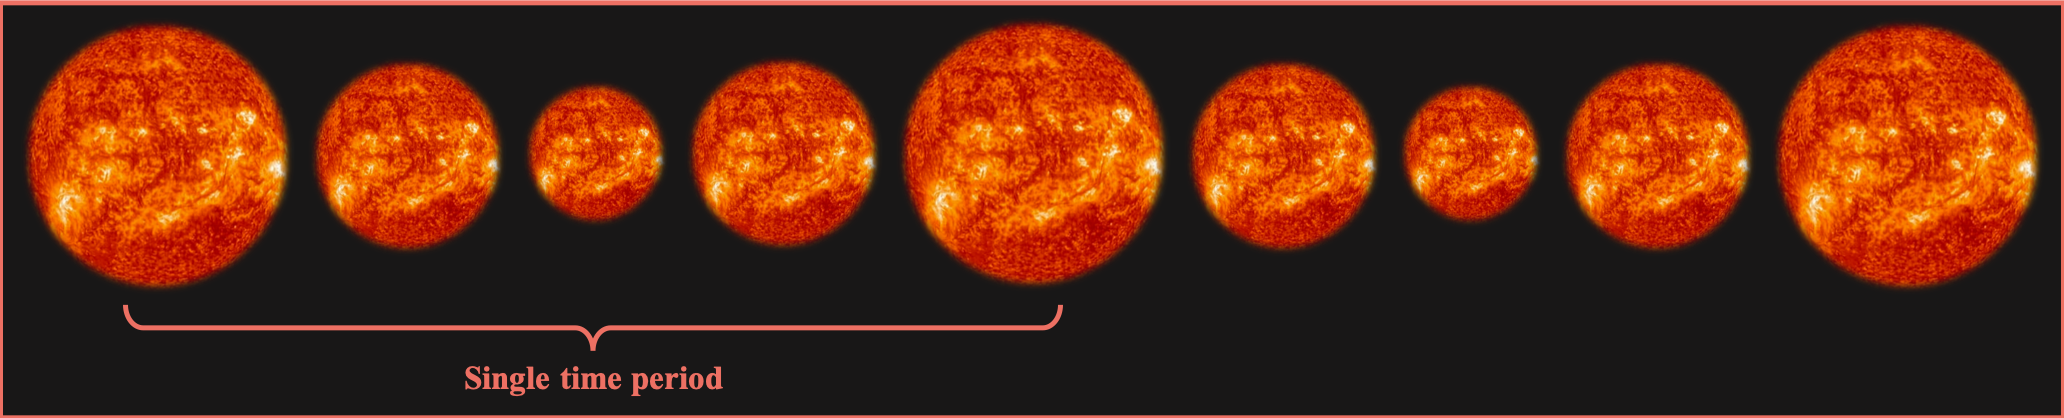
\includegraphics[width=0.95\textwidth]{Images/cepheid-period.png}
        \textbf{
            \caption{Cepheid variable stars expand and contract with a regular time-period.}
        }
        \end{center}
        \label{cepheid-period}
        \vspace*{8in}
    \end{figure}
    %---\figure--- 
    
%----------\1. STAR CLUSTERS----------
%
%
%
%
%
\clearpage
%
%
%
%
%
%-----2. INTRODUCTION TO SCIENCE-----
\invisiblesection{2. Scientific Research}
    
    %---title---
    \begin{tcolorbox}[enhanced,colback=dblue!80!black,colframe=dblue!80!black,drop fuzzy shadow]
    \begin{center}  
    {\color{white}
        \huge{\textbf{2. SCIENTIFIC RESEARCH}}
    }
    \end{center}
    \end{tcolorbox}
    %---\title---
    
    
    
    %---intro box---
    \begin{tcolorbox}[enhanced,colback=dblue!60!white,colframe=dblue!80!black]
    {\color{white}
        \textbf{After reading this section, you will be able to answer these questions:}
        \begin{itemize}
        \renewcommand\labelitemi{--}
            \item \textbf{What exactly is ‘scientific research'?}
            \item \textbf{How do scientists produce important conclusions from results that are extracted from scientific research?}
            \item \textbf{How does the ongoing nature of scientific research span generations?}
        \end{itemize}
    }
    \end{tcolorbox}
    %---\intro box---
    
    
    
    
    
    %---enumerate 1,2---
    \begin{enumerate}[label=\color{dblue}\theenumi]
            \item Science and scientific discovery can be generally split into  a three step process from start to finish (\textbf{figure \ref{scientific-process}}).
            
            
            \begin{itemize}[label=\textcolor{dblue}{\textbullet}]
                \item In this project, you will experiment with tools that Astronomers use to test their scientific hypotheses with.
            \end{itemize}
    \end{enumerate}
    %---\enumerate---
    
    

    %---figure 2--- 
    \begin{figure}[h]
        \centering
        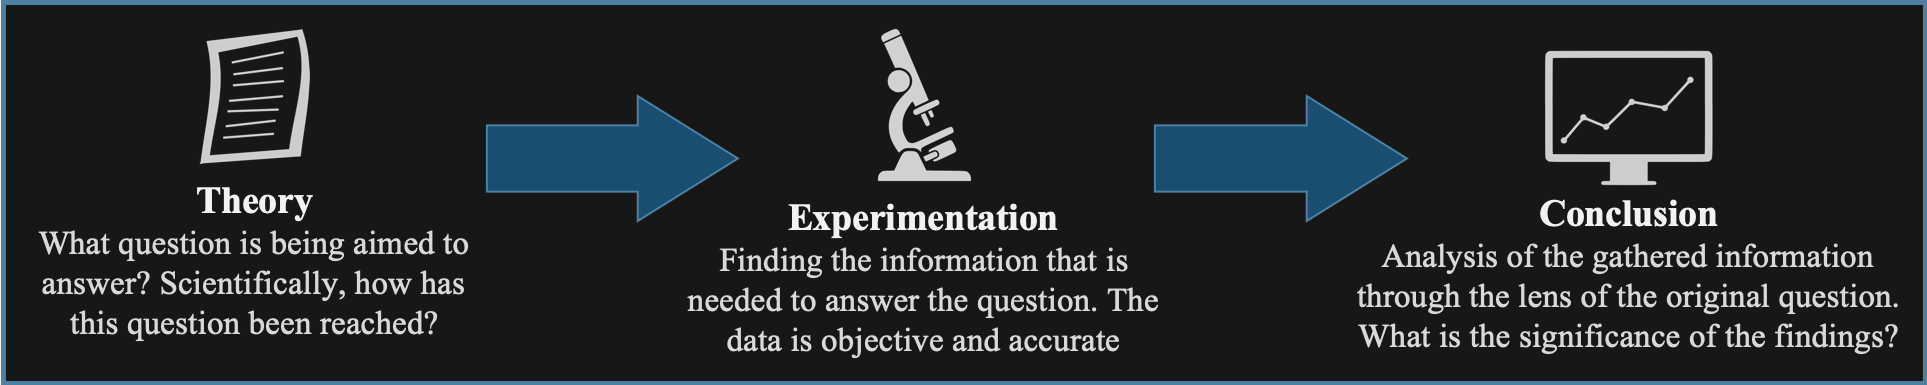
\includegraphics[width=1\textwidth]{Images/theory-etc.png}
        \textbf{
            \caption{Methodology for the general scientific process. Most, if not all scientific discoveries made throughout history followed this process.}
        }
        \label{scientific-process}
    \end{figure}
    %---\figure--- 
    
    
    %---figure 3---
    \begin{figure}[h]
        \centering
        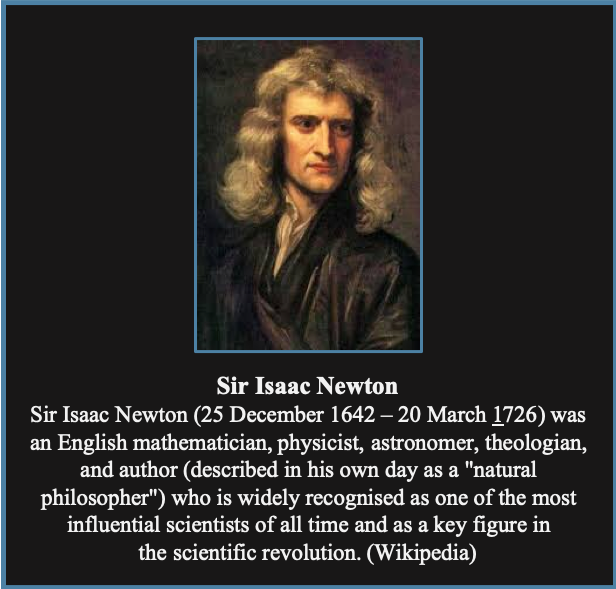
\includegraphics[width=0.6\textwidth]{Images/newton.png}
        \textbf{
            \caption{Sir Isaac Newton.}
        }
        \label{newton}
    \end{figure}
    %---\figure---
    
    
    %---colourbox 2---
    \begin{tcolorbox}[colback=white,colbacktitle=dblue!75!white,colframe=dblue!75!white,title=\textbf{Science is creative! Here is an example.}]
    
        \renewcommand{\theenumi}{\Alph{enumi}}
        \begin{enumerate}
            \item Take the example of finding the acceleration due to gravity, $ \textcolor{red}{\boldsymbol{g}} $. Finding Earth's gravitational acceleration can be determined through a simple experiment - dropping a ball.\\
            
            This is a straight-forward experiment. Imagine that you are the first person to ever think of attempting this experiment, before even knowing what gravity is or how it works. How would you do this?
            
            
            \begin{itemize}
                \item \textbf{Theory.} The key relationship which informs this experiment is that \emph{\textcolor{purple}{speed is equal to distance divided by time}} for an object moving with constant speed. \\
                
                Differentiating this relationship, we find that \emph{\textcolor{purple}{acceleration is proportional to distance divided by time squared}} ($ \textcolor{red}{\boldsymbol{acceleration \equiv ms^{-2}}} $) for an object moving with constant acceleration.\\
                
                If this acceleration relationship is found true for falling objects, then this implies that a constant acceleration exists on Earth's surface in the downwards direction (towards the centre of the Earth). \\
                
                This forms our hypothesis (\emph{\textcolor{purple}{if x is shown, then y is true}}).\\
                    
                    
                \item \textbf{Experimentation.} So to find $ \textcolor{red}{\boldsymbol{g}} $, drop a ball over a range of known distances, $ \textcolor{red}{\boldsymbol{s}} $, and measure the time that it takes to drop these distances, $ \textcolor{red}{\boldsymbol{t}} $. What would happen if, instead of letting the ball free-fall, the ball was let to fall down inclined planes of the same distances? Is it worth experimenting with this to improve the validity of the experiment? These are useful questions to ask whilst devising the experiment.\\
                
                In order to \emph{\textcolor{purple}{reduce error}} (or \emph{\textcolor{purple}{increase accuracy}}), take \emph{\textcolor{purple}{repeat measurements}} of $ \textcolor{red}{\boldsymbol{t}} $. It is important to think about how to reduce error in any measurements that are taken - taking repeat measurements is just one method of doing this.\\


                \item \textbf{Conclusion.} Plotting distance against time squared shows a linear relationship. So a constant acceleration exists at Earths surface. Re-arranging the 'SUVAT' equation $ \textcolor{red}{\boldsymbol{s = ut + 1/2 at^2}} $, the acceleration due to gravity can be calculated.
                
                    \begin{center}
                        $ \textcolor{red}{\boldsymbol{g=9.81ms^{-2}}} $.\\
                    \end{center}
                        
                So, what exactly is \emph{\textcolor{purple}{concluded}} from this experiment?
                
                    \renewcommand{\theenumi}{\roman{enumi}}
                    \begin{enumerate} 
                    
                        \item From this same conceptual experiment, Sir Isaac Newton (\textbf{figure 3}) famously concluded years of scientific research with his laws of gravitation. This is a fundamental block of Physics and is referred to by students and scientists everyday. 
                        
                        \item A \emph{\textcolor{purple}{larger error}} in the results causes the experiment to be \emph{\textcolor{purple}{less accurate}}.
                        
                    \end{enumerate} 
                    
                
            \end{itemize}
            
        \end{enumerate}
        
    \end{tcolorbox}
    %---\colourbox---
    
%----------\2. INTRODUCTION TO SCIENCE----------
%
%
%
%
%
\clearpage
%
%
%
%
%
%-----3. DISTANCE OF STARS-----
\invisiblesection{3. Cepheids}
    
    %---title---
    \begin{tcolorbox}[enhanced,colback=turquoise!80!black,colframe=turquoise!80!black,drop fuzzy shadow]
    \begin{center}  
    {\color{white}
        \Huge{\textbf{3. THE DISTANCE OF STARS}}
    }
    \end{center}
    \end{tcolorbox}
    %---\title---
    
    
    
    %---intro box---
    \begin{tcolorbox}[enhanced,colback=turquoise!95!white,colframe=turquoise!80!black]
    {\color{white}
        \textbf{After reading this section, you will be able to answer these questions:}
        \begin{itemize}
        \renewcommand\labelitemi{--}
            \item \textbf{}
        \end{itemize}
    }
    \end{tcolorbox}
    %---\intro box---

    
    
    
    
    %---enumerate 1-6---
    \begin{enumerate}[label=\color{turquoise}\theenumi]

        %\begin{center}
        %\begin{tabular}{ |c|c| } 
        %    \hline
        %    Pearl Cluster & C1 Pinnea \\
        %    \hline
        %    cell5 & cell6 \\ 
        %    \hline
        %    cell7 & cell8 & cell9 \\ 
        %    \hline
        %\end{tabular}
        %\end{center}
        

        \item For this project, you are going to work with a fictional open star cluster called the \emph{\textcolor{turquoise}{Pearl Cluster}}.
        
        \item Suppose that you can see the Pearl Cluster in the sky, and you'd like to find how far away it is - it's distance. How are we to find this out? 
        
        \item In 1912 astronomer Henrietta Swan Leavitt (\textbf{figure \ref{henswanlev}}) discovered a fascinating relationship between the \emph{\textcolor{turquoise}{pulsation time period}} and the \emph{\textcolor{turquoise}{luminosity}} of \emph{\textcolor{turquoise}{Cepheid variable stars}}.
        
        \item Thanks to Henrietta Swan Leavitt's work, we can use the properties of Cepheid variable stars to estimate their distances away from us on Earth. 
        
        \item If we are lucky enough to observe one of these Cepheid variable stars amongst the Pearl Cluster, then this could help us \emph{\textcolor{turquoise}{estimate}} the distance to the entire Pearl cluster.
        
        \item Below, we will discuss how Henrietta Swan Leavitt was able to determine the distances to Cepheid variable stars using only their pulsation properties.
        
        
    \end{enumerate}
    %---\enumerate---
    
    
    
    %---figure 1---
    \begin{figure}[h!]
        \centering
        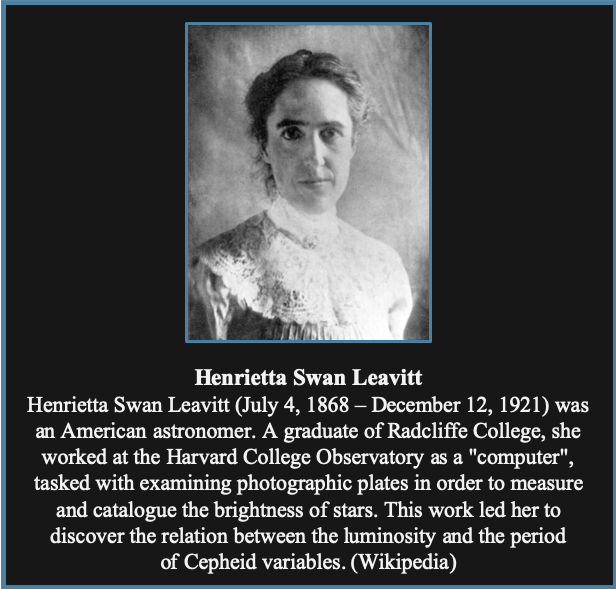
\includegraphics[width=0.4\textwidth]{Images/henswanlev.png}
        \textbf{
            \caption{Henrietta Swan Leavitt.}
        }
        \label{henswanlev}
    \end{figure}
    %---\figure---
    
    
    
    %---colour box 1---
    \begin{tcolorbox}[enhanced jigsaw,breakable,pad at break*=1mm,colback=white,colbacktitle=turquoise!75!white,colframe=turquoise!75!white,title=\textbf{Henrietta Swan Leavitt discovered that Cepheid variable stars can act as distance 'markers' in the Universe.}]
    
        \renewcommand{\theenumi}{\Alph{enumi}}
        \begin{enumerate}
            \item Henrietta Swan Leavitt discovered how to calculate the distance to Cepheid variable stars. 
            \item Swan Leavitt showed that there is a \emph{\textcolor{turquoise}{direct proportionality relationship}} between the \emph{\textcolor{turquoise}{brightness}} and the \emph{\textcolor{turquoise}{logarithm of the period}} of Cepheid variable stars.
            
            \begin{itemize}
                \item In other words:
                                            
                    \begin{center}
                           
                            $ \textcolor{red}{\boldsymbol{B}} $ \propto \textcolor{red}{\boldsymbol{log(P)}}

                    \end{center}
                    
            \end{itemize}
            
        \end{enumerate}
        
                %---colour box 1 inside colour box 2---
                \begin{tcolorbox}[enhanced jigsaw,breakable,pad at break*=1mm,colback=dblue!5!white,colframe=dblue!75!white,colbacktitle=dblue!75!white,title=\textbf{We can explore this relationship further.},drop fuzzy shadow]
                
                    % B log(P) relationship graph
                    % absolute and apparent magnitude
                    % introduce Cepheid C1 Pinnea within Pearl Cluster
                        % with M and m given
                    
                \end{tcolorbox}
                %---\colour box---
                %
                %---colour box 2 inside colour box 2---
                \begin{tcolorbox}[enhanced jigsaw,breakable,pad at break*=1mm,colback=red!5!white,colframe=red!75!white,colbacktitle=red!75!white,title=\textbf{We can explore this relationship further.},drop fuzzy shadow]
                
                    \renewcommand{\theenumi}{\Roman{enumi}}
                    \begin{enumerate}
                        \item Within the \emph{\textcolor{turquoise}{Pearl Cluster}} is a Cepheid named \emph{\textcolor{turquoise}{C1 Pinnea}}. If we can find the distance to this Cepheid variable star, we can estimate the distance to the \textbf{\textcolor{red}{Pearl cluster}}. The period-luminosity relationship allows us to do this.
                        
                        \begin{itemize}
                            \item The fictional Cepheid variable star which is observed to be near the \textbf{\textcolor{red}{Pearl cluster}} is \textbf{\textcolor{red}{C1 Pinnea}}.
                            \item From Earth, we can only measure the apparent magnitude, $ \textcolor{red}{\boldsymbol{m}} $, and the period, $ \textcolor{red}{\boldsymbol{P}} $ of \textbf{\textcolor{red}{C1 Pinnea}}.
                            
                            \item Using Henrietta Swan Leavitt's period-luminosity graph (\textbf{figure \ref{per-lum}}), we can \emph{\textcolor{purple}{interpolate}} to find the absolute magnitude, $ \textcolor{red}{\boldsymbol{M}} $.
                        \end{itemize}
                        
                        
                        \item The \emph{\textcolor{purple}{magnitude scale}} is a scale that Astronomers use to measure the brightness of stars:\\

                                \begin{center}
                               
                                    $ \textcolor{red}{\boldsymbol{m}} $ = {\emph{\textcolor{purple}{Apparent magnitude}}} = A measurement of the ‘brightness' of a star as measured from Earth.

                                    $ \textcolor{red}{\boldsymbol{M}} $ = {\emph{\textcolor{purple}{Absolute magnitude}}} = A measurement of the ‘brightness' of a star as measured from exactly 10pc away.

                                \end{center}
                            
                        \item Using this equation, called the \emph{\textcolor{purple}{distance-modulus formula}}, we can therefore find the distance of the \textbf{\textcolor{red}{C1 Pinnea}} from Earth.
                        
                            \begin{center}
                               
                                $ \textcolor{red}{\boldsymbol{d=10*10^{\frac{m-M}{5}}}} $
                                
                            \end{center}
                        
                        \item We now have an estimation of the distance to the \textbf{\textcolor{red}{Pearl cluster}} by using \textbf{\textcolor{red}{C1 Pinnea}} as a marker!
                    \end{enumerate}
                    
                \end{tcolorbox}
                %---\colour box ---
            
    \end{tcolorbox}
    %---\outer colour box---
    
%-----\3. DISTANCE TO STARS-----
%
%
%
%
%
\clearpage
%
%   
%   
%
%   
%-----4. THE HR DIAGRAM-----
\invisiblesection{4. The Hertzsprung-Russel (HR) Diagram}

    %---title 3---
    \begin{tcolorbox}[enhanced,colback=dgreen!80!black,colframe=dgreen!80!black,drop fuzzy shadow]
    \begin{center}  
    {\color{white}
        \huge{\textbf{4. THE HERTZSPRUNG-RUSSEL DIAGRAM}}
    }
    \end{center}
    \end{tcolorbox}
    %---\title 3---
    
    
    
    %---intro box 3---
    \begin{tcolorbox}[enhanced,colback=dgreen!80!white,colframe=dgreen!80!black]
    {\color{white}
        \textbf{In this section these questions will be answered.}
        \begin{itemize}
        \renewcommand\labelitemi{--}
            \item \textbf{There are over ten billion stars in the Galaxy. How are they all categorised?}
            \item \textbf{How did science and data the Hertzsprung-Russell diagram develop?}
            \item \textbf{Why is categorising stars necessary?}
        \end{itemize}
    }
    \end{tcolorbox}
    %---\intro box 3---
    
    
    
    %---figure 3.1---
    \begin{figure}[h!]
        \centering
        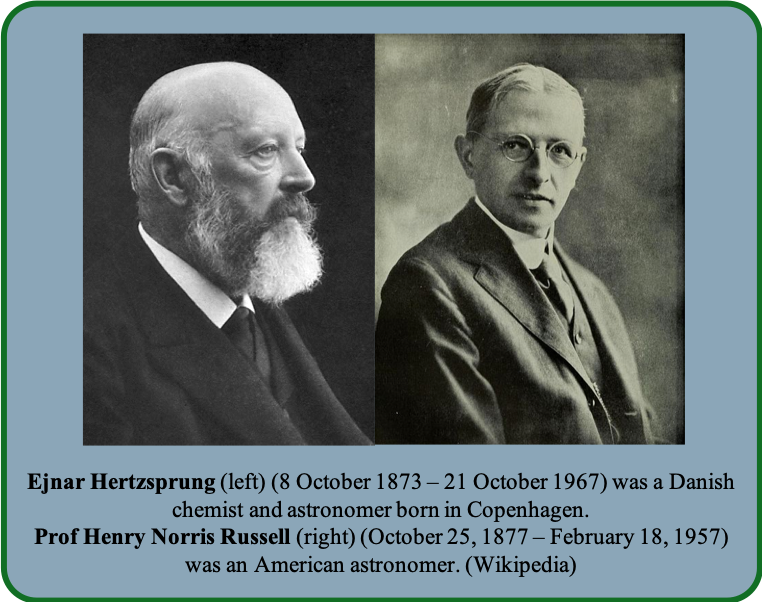
\includegraphics[width=0.4\textwidth]{Images/hertzsprung-russell.png}
        \caption{Ejnar Hertzsprung and Henry Norris Russell.}
        \label{hertz-russell}
    \end{figure}
    %---\figure 3.1---



    %---enumerate 3.12---
    \begin{enumerate}[label=\color{dgreen}\theenumi]
        \item In the early 1900's, whilst analysing the data of a range of stars, Ejnar Hertzsprung and Henry Norris Russell decided to plot the \emph{\textcolor{dblue}{luminosity of the stars against their temperatures}}.
        
        \item This graph which plotted luminosity on the vertical y-axis and temperature on the horizontal x-axis became known as the \emph{\textcolor{dblue}{Hertzsprung-Russel diagram}} (the \emph{\textcolor{dblue}{HR diagram}} for short).
    \end{enumerate}
    %---\enumerate 3.12---
    
    
    
    %---figure 3.2---
    \begin{figure}[h!]
        \centering
        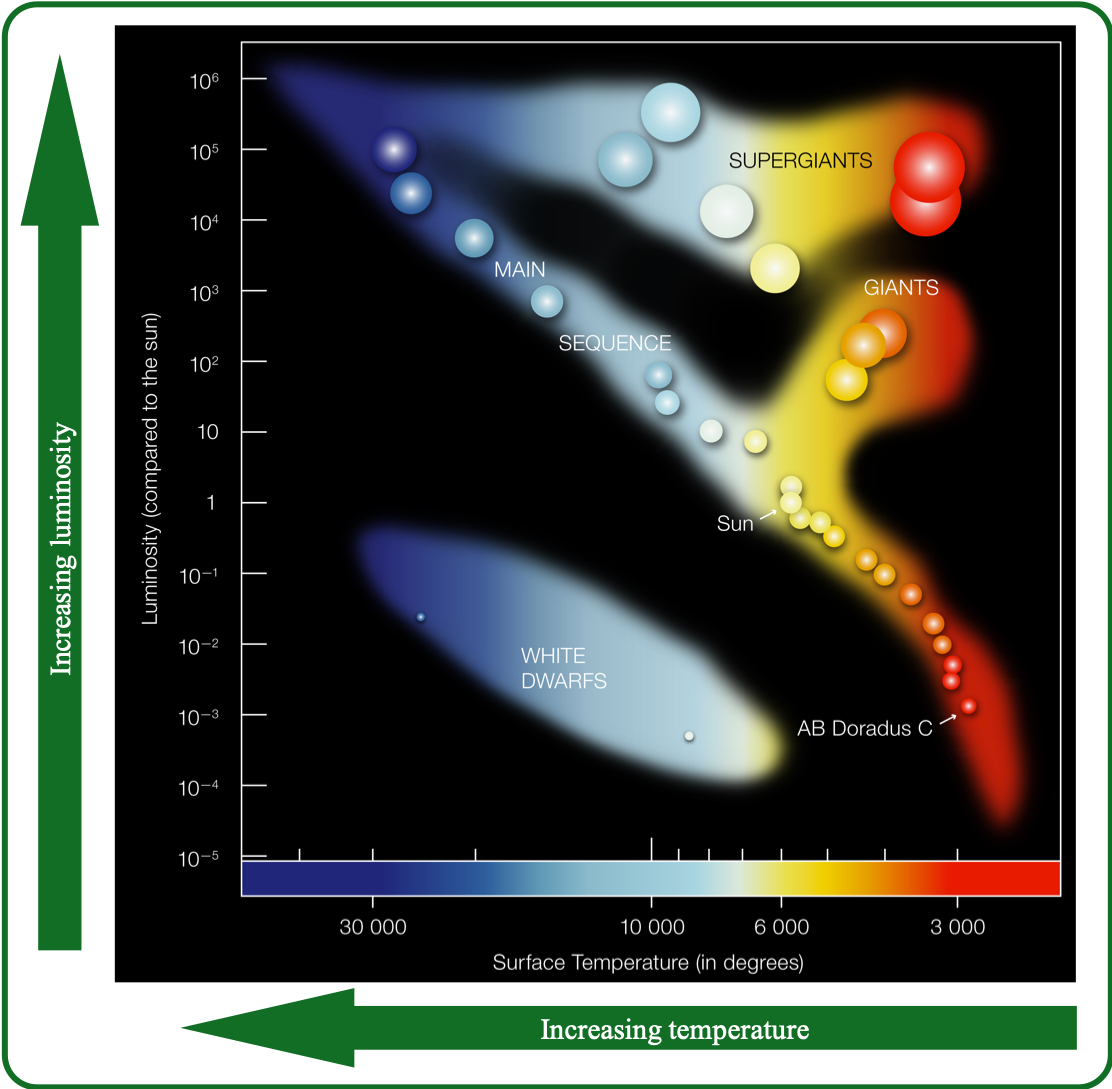
\includegraphics[width=0.45\textwidth]{Images/hrd.png}
        \caption{The Hertzsprung-Russel diagram categorises stars over their life-cycle.}
        \label{hrd}
    \end{figure}
    %---\figure 3.2---
    
    
    
    %---colour box 3.1---
    \begin{tcolorbox}[colback=white,colbacktitle=dgreen!75!white,colframe=dgreen!75!white,title=\textbf{HR-diagrams tell us at what stage in their life cycles stars are}]
    
        \begin{itemize}
            \item The \emph{\textcolor{dblue}{HR diagram}} shows us a timeline of how stars evolve and age in terms of their temperature and luminosity.
            
            
                \renewcommand{\theenumi}{\alph{enumi}}
                \begin{enumerate}
                    \item Look at the HR diagram above which displays a range of stars in the \emph{\textcolor{dblue}{main sequence}} stage in their life cycles. Our Sun is also in its main sequence stage.
        
                    \item The main sequence is called the main sequence because it is the section of stellar evolution that stars spend the majority spend the majority of their time before evolving into a different stage.
                \end{enumerate}
    
    
            \item After a star concludes its main sequence path, it will evolve into the next stage of its life. Stars of different masses/internal properties will evolve differently, and can be imaged on the HR diagram.
        \end{itemize}
        
    \end{tcolorbox}
    %---\colour box 3.1---
        
        
        
    %---enumerate 3.3---    
    \begin{enumerate}[label=\color{dgreen}\theenumi]
    \setcounter{enumi}{2}
        \item The table below shows the different evolutionary paths that stars can take after the main sequence.
    \end{enumerate}
    %---\enumerate 3.3--- 

    
    
    %---enumerate 3.4---    
    \begin{enumerate}[label=\color{dgreen}\theenumi]
    \setcounter{enumi}{3}
        \item When representing star clusters on HR diagrams, each \emph{\textcolor{dblue}{individual star}} in the star cluster is mapped as an \emph{\textcolor{dblue}{individual point}} on the temperature-luminosity graph
    \end{enumerate}  
    %---\enumerate 3.4---  
        
       
       
    %---figure 3.3---   
    \begin{figure}[h!]
        \centering
        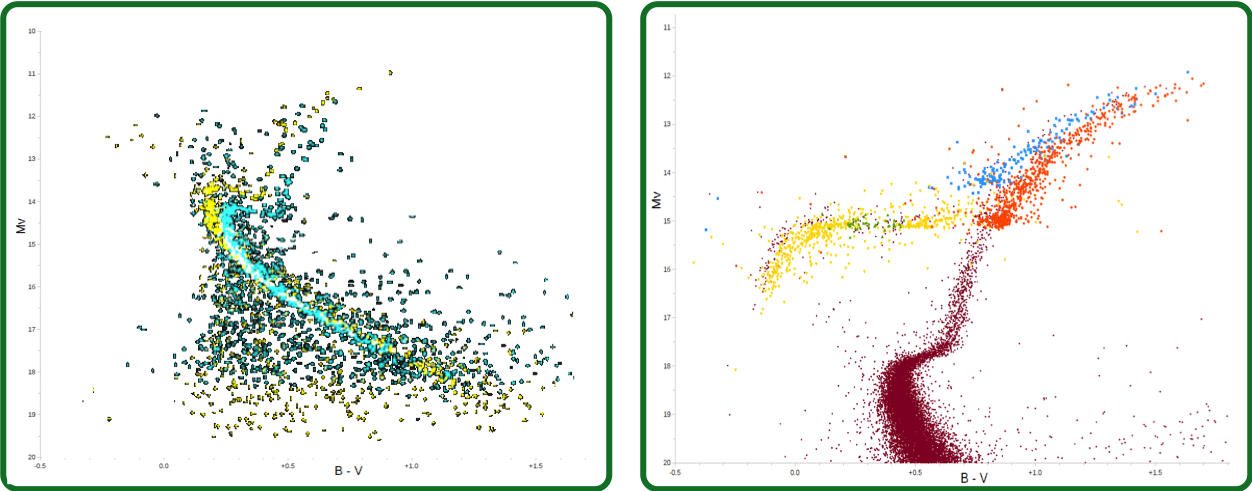
\includegraphics[width=0.8\textwidth]{Images/glob-open-hrd.png}
        \caption{The Hertzsprung-Russel diagram for open (left) and globular (right) star clusters.}
        \label{hr-glob-open}
    \end{figure}
    %---\figure 3.3--- 
    
    
    
    %---colour box 3.2---
    \begin{tcolorbox}[enhanced,colback=dgreen!80!white,colframe=dgreen!80!black]
    {\color{white}
        \textbf{By looking at the HR-diagrams for both open and globular clusters, what can you determine about the relative ages of both of these types of clusters?}\\
        \textbf{Fill in the table to describe the differences between open and globular clusters. You may want to think about relative; age, mass, size and chemical composition. Use books or the internet to find your information.}
    }
    \end{tcolorbox}
    %---\colour box 3.2---



    %---table 3.1---
    \begin{tabularx}{1\textwidth} { 
           >{\raggedcenter\arraybackslash}X
          | >{\raggedcenter\arraybackslash}X  }
         \hline
         \Large\textbf{\textcolor{dgreen}{Open Cluster}} & \Large\textbf{\textcolor{dgreen}{Globular Cluster}}  \\
         \hline
           &   \\
           &   \\
           &   \\
           &   \\
       &   \\
    \end{tabularx}
    %---\table 3.1---
   


%-----\3. THE HR DIAGRAM-----
%
%
%
%
%
\newpage
%
%
%
%
%
%-----4. ISOCHRONES-----
\invisiblesection{4. How old are star clusters?}

    %---title 4---
    \begin{tcolorbox}[enhanced,colback=purple!80!black,colframe=purple!80!black,drop fuzzy shadow]
    \begin{center}  
    {\color{white}
        \Huge{\textbf{4. ISOCHRONES AND STELLAR AGES}}
    }
    \end{center}
    \end{tcolorbox}
    %---\title 4---
    
    
    
    %---intro box 4---
    \begin{tcolorbox}[enhanced,colback=purple!80!white,colframe=purple!80!black]
    {\color{white}
        \textbf{In this section these questions will be answered.}
        \begin{itemize}
        \renewcommand\labelitemi{--}
            \item \textbf{Using the Hertzsprung-Russell diagram, how can we estimate the age of star clusters?} 
            \item \textbf{How can computing help scientist simplify complex calculations (\emph{activity 2})?}
        \end{itemize}
    }
    \end{tcolorbox}
    %---\intro box 4---
    
    
    
    
    
    %---enumerate 4.12---
    \begin{enumerate}[label=\color{purple}\theenumi]
        \item Stars and star clusters are very old. Star clusters, like most other things in the Universe, are \emph{\textcolor{red}{a few billion years old}}.
        
        \item We can be more specific than this though, and calculate the specific age of star clusters in the Universe using \emph{\textcolor{red}{star cluster HR diagrams}}.
    \end{enumerate}
    %---\enumerate 4.12---
    
    
    
    %---figure 4.1---
    \begin{figure}[h!]
        \centering
        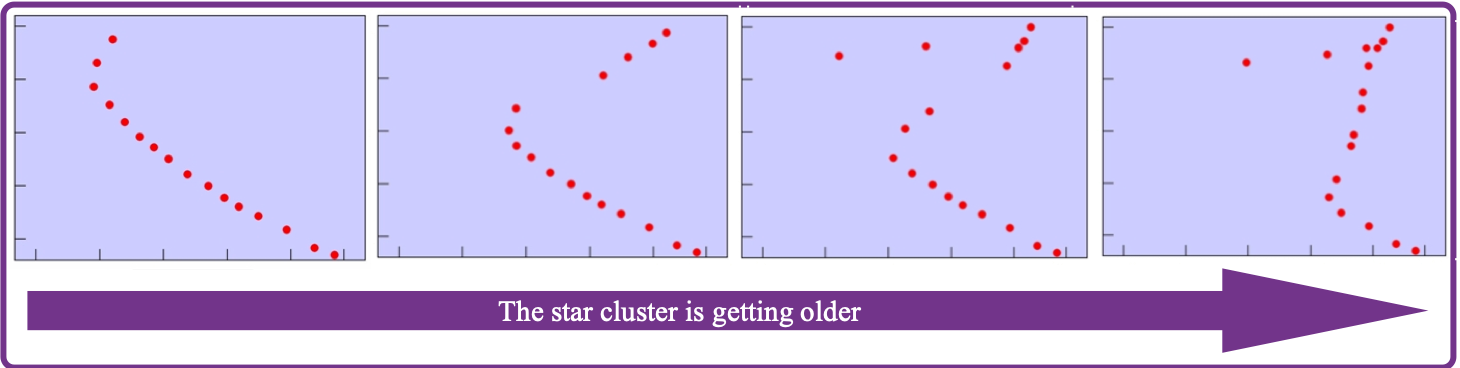
\includegraphics[width=0.9\textwidth]{Images/isochrone-age.png}
        \caption{Isochrones allow us to see how old star clusters are.}
        \label{iso-age}
    \end{figure}
    %---\figure 4.1---
    
    
    
    %---colour box 4.1---
    \begin{tcolorbox}[colback=white,colbacktitle=purple!75!white,colframe=purple!75!white,title=\textbf{We can use HR-diagrams of star clusters to calculate their age.}]
    
        \begin{itemize}
            \item The HR-diagram shows the evolution of stars over their life cycle. In other words, stars on a HR-diagram change their position in relation to their \emph{\textcolor{red}{age}}.
            
            
            \begin{itemize}
                \item On the main-sequence line of the HR-diagram, each plot point shows a star at the different stage of their evolutionary cycle (or age). As stars get older, they begin to move up the main-sequence and evolve to other sections, their path depending on their mass.
            \end{itemize}
            
            
            \item Isochrones on the other hand show how a \emph{\textcolor{red}{population}} of stars with varying \emph{\textcolor{red}{masses}} of the \emph{\textcolor{red}{same age}} evolve. An isohchrone for a young group of stars will look different to an isochrone for a younger group of stars.
            
            \item In this case, isochrones act as markers that groups of stars with unknown ages can be compared against - the age of a star cluster can be determined by which aged isochrone it has the least difference with.
        \end{itemize}
        
    \end{tcolorbox}
    %---\colour box 4.1---



    %---enumerate 4.3---
    \begin{enumerate}[label=\color{purple}\theenumi]
    \setcounter{enumi}{2}
        \item If we plot a population (remember that 'population' means a group of \emph{\textcolor{red}{varying masses}}) of stars on a HR-diagram, we can extract the points of the same age of each evolution path (each mass star) to create a range of isochrones (activity 2).
    \end{enumerate}
    %---\enumerate 4.3---
    
    

%-----\4. ISOCHRONES-----



\end{document}